\ifx\allfiles\undefined
\documentclass[12pt, a4paper,oneside, UTF8]{ctexbook}
\usepackage[dvipsnames]{xcolor}
\usepackage{mathtools}   % 数学公式(mathtools 是 amsmath 的上位替代)
\usepackage{amsthm}    % 定理环境
\usepackage{amssymb}   % 更多公式符号
\usepackage{graphicx}  % 插图
%\usepackage{mathrsfs}  % 数学字体
%\usepackage{newtxtext,newtxmath}
%\usepackage{arev}
\usepackage{kmath,kerkis}
\usepackage{newtxtext}
\usepackage{bbm}
\usepackage{enumitem}  % 列表
\usepackage{geometry}  % 页面调整
%\usepackage{unicode-math}
\usepackage[colorlinks,linkcolor=black]{hyperref}

\usepackage{wrapfig}


\usepackage{ulem}	   % 用于更多的下划线格式,
					   % \uline{}下划线,\uuline{}双下划线,\uwave{}下划波浪线,\sout{}中间删除线,\xout{}斜删除线
					   % \dashuline{}下划虚线,\dotuline{}文字底部加点


\graphicspath{ {flg/},{../flg/}, {config/}, {../config/} }  % 配置图形文件检索目录
\linespread{1.5} % 行高

% 页码设置
\geometry{top=25.4mm,bottom=25.4mm,left=20mm,right=20mm,headheight=2.17cm,headsep=4mm,footskip=12mm}

% 设置列表环境的上下间距
\setenumerate[1]{itemsep=5pt,partopsep=0pt,parsep=\parskip,topsep=5pt}
\setitemize[1]{itemsep=5pt,partopsep=0pt,parsep=\parskip,topsep=5pt}
\setdescription{itemsep=5pt,partopsep=0pt,parsep=\parskip,topsep=5pt}

% 定理环境
% ########## 定理环境 start ####################################
\theoremstyle{definition}
\newtheorem{defn}{\indent 定义}[section]

\newtheorem{lemma}{\indent 引理}[section]    % 引理 定理 推论 准则 共用一个编号计数
\newtheorem{thm}[lemma]{\indent 定理}
\newtheorem{corollary}[lemma]{\indent 推论}
\newtheorem{criterion}[lemma]{\indent 准则}

\newtheorem{proposition}{\indent 命题}[section]
\newtheorem{example}{\indent \color{SeaGreen}{例}}[section] % 绿色文字的 例 ,不需要就去除\color{SeaGreen}{}
\newtheorem*{rmk}{\indent \color{red}{注}}

% 两种方式定义中文的 证明 和 解 的环境:
% 缺点:\qedhere 命令将会失效【技术有限,暂时无法解决】
\renewenvironment{proof}{\par\textbf{证明.}\;}{\qed\par}
\newenvironment{solution}{\par{\textbf{解.}}\;}{\qed\par}

% 缺点:\bf 是过时命令,可以用 textb f等替代,但编译会有关于字体的警告,不过不影响使用【技术有限,暂时无法解决】
%\renewcommand{\proofname}{\indent\bf 证明}
%\newenvironment{solution}{\begin{proof}[\indent\bf 解]}{\end{proof}}
% ######### 定理环境 end  #####################################

% ↓↓↓↓↓↓↓↓↓↓↓↓↓↓↓↓↓ 以下是自定义的命令  ↓↓↓↓↓↓↓↓↓↓↓↓↓↓↓↓

% 用于调整表格的高度  使用 \hline\xrowht{25pt}
\newcommand{\xrowht}[2][0]{\addstackgap[.5\dimexpr#2\relax]{\vphantom{#1}}}

% 表格环境内长内容换行
\newcommand{\tabincell}[2]{\begin{tabular}{@{}#1@{}}#2\end{tabular}}

% 使用\linespread{1.5} 之后 cases 环境的行高也会改变,重新定义一个 ca 环境可以自动控制 cases 环境行高
\newenvironment{ca}[1][1]{\linespread{#1} \selectfont \begin{cases}}{\end{cases}}
% 和上面一样
\newenvironment{vx}[1][1]{\linespread{#1} \selectfont \begin{vmatrix}}{\end{vmatrix}}

\def\d{\textup{d}} % 直立体 d 用于微分符号 dx
\def\R{\mathbb{R}} % 实数域
\def\N{\mathbb{N}} % 自然数域
\def\C{\mathbb{C}} % 复数域
\def\Z{\mathbb{Z}} % 整数环
\def\Q{\mathbb{Q}} % 有理数域
\newcommand{\bs}[1]{\boldsymbol{#1}}    % 加粗,常用于向量
\newcommand{\ora}[1]{\overrightarrow{#1}} % 向量

% 数学 平行 符号
\newcommand{\pll}{\kern 0.56em/\kern -0.8em /\kern 0.56em}

% 用于空行\myspace{1} 表示空一行 填 2 表示空两行  
\newcommand{\myspace}[1]{\par\vspace{#1\baselineskip}}

%s.t. 用\st就能打出s.t.
\DeclareMathOperator{\st}{s.t.}

%罗马数字 \rmnum{}是小写罗马数字, \Rmnum{}是大写罗马数字
\makeatletter
\newcommand{\rmnum}[1]{\romannumeral #1}
\newcommand{\Rmnum}[1]{\expandafter@slowromancap\romannumeral #1@}
\makeatother
\begin{document}
	% \title{{\Huge{\textbf{$Partial \,\, Differential \,\, Equations$}}}\footnote{参考书籍:\\
			\hspace*{4em} \textbf{《Partial Differential Equations》 -- Lawrence C. Evans} \\
			\hspace*{4em} \textbf{《Partial Differential Equations》 -- Fritz John} \\
			\hspace*{4em} \textbf{《数学物理方程讲义 (第二版)》--  姜礼尚、陈亚浙、刘西垣、易法槐} 
			}}
\author{$-TW-$}
\date{\today}
\maketitle                   % 在单独的标题页上生成一个标题

\thispagestyle{empty}        % 前言页面不使用页码
\begin{center}
	\Huge\textbf{序}
\end{center}


\vspace*{3em}
\begin{center}
	\large{\textbf{天道几何,万品流形先自守;}}\\
	
	\large{\textbf{变分无限,孤心测度有同伦。}}
\end{center}

\vspace*{3em}
\begin{flushright}
	\begin{tabular}{c}
		\today \\ \small{\textbf{长夜伴浪破晓梦,梦晓破浪伴夜长}}
	\end{tabular}
\end{flushright}


\newpage                      % 新的一页
\pagestyle{plain}             % 设置页眉和页脚的排版方式(plain:页眉是空的,页脚只包含一个居中的页码)
\setcounter{page}{1}          % 重新定义页码从第一页开始
\pagenumbering{Roman}         % 使用大写的罗马数字作为页码
\tableofcontents              % 生成目录

\newpage                      % 以下是正文
\pagestyle{plain}
\setcounter{page}{1}          % 使用阿拉伯数字作为页码
\pagenumbering{arabic}
\setcounter{chapter}{0}    % 设置 -1 可作为第零章绪论从第零章开始 
	\else
	\fi
	%  ############################ 正文部分
\chapter{Prologue}
\section{Partial Differential Equations}
	下面我们给出\textbf{偏微分方程 (PDE)}的定义.
	\begin{defn}\label{def 1.1.1}
		An expression of the form
		\[ F(D^k u , D^{k - 1}u , \cdots , Du , u , x) = 0 , \,\, x \in U \subset \R^n \]
		is called a \underline{\textcolor{blue}{\textbf{$k^{th}$-order partial differential equation}}}, where
		\[ F : \R^{n^{k}} \times \R^{n^{k - 1}} \times \cdots \times \R^n \times \R \times U \longrightarrow \R \]
		and
		\[ u : U \subset \R^n \longrightarrow \R \]
		
		\vspace*{2em}
		
		\begin{rmk}
			\begin{itemize}
				\item 此处的函数$u$ 未必$k$ 阶连续可微, 因此其$k$ 阶偏导的偏导算子不一定能交换次序, 故符号$D^{k}u$ 中包含了$n^k$ 种$k$ 阶偏导.
				
				\vspace{2em}
				
				\item \textbf{[高阶偏导数计数问题]}. 对于$u \in C^k$, 此时$k$ 阶偏导算子可任意交换次序, 则对于符号$D^k u$, 其代表了几种$k$ 阶偏导数?
				
				\vspace{2em}
				
				\begin{solution}
					即考虑$D^{\alpha} u (\left| \alpha \right| = k)$ 的种数. 可转化为求非负数不定方程
					\[ \alpha_1 + \alpha_2 + \cdots + \alpha_n = k \]
					的解的个数的问题, 其中$\alpha_i$ 表示$u$ 对自变量$x$ 的第$i$ 个分量所求偏导阶数, 即$(\dfrac{\partial}{\partial x_i})^{\alpha_i}$. \\
					利用\textbf{插板法}, 往$k$ 个球插入$n - 1$ 个板即可得到$n$ 份, 球和板共$k + n - 1$ 个, 即可视作往$k + n - 1$ 个空位中任意排列$k$ 个球和$n - 1$ 个板, 即有
					\[ {k + n - 1 \choose k} = {k + n - 1 \choose n - 1} \text{种}  \]
				\end{solution}
			\end{itemize}
		\end{rmk}
	\end{defn}
	
	\vspace{6em}	
	
	下面给出\textbf{偏微分方程 (PDE)} 的一些\textbf{线性}的概念.
	\begin{defn}\label{def 1.1.2}
		\begin{itemize}
			\item The PDE is called \underline{\textcolor{blue}{\textbf{linear}}} if it has the form
			\[ \sum_{\left| \alpha \right| \leq k} a_{\alpha}(x) D^{\alpha}u = f(x) \]
			for given $a_\alpha$ and $f$. Moreover, it is called \underline{\textcolor{blue}{\textbf{homogenuous (齐次)}}} if $f \equiv 0$.
			
			\vspace{2em}
			
			\item The PDE is \underline{\textcolor{blue}{\textbf{semilinear}}} if it has the form
			\[ \sum_{\left| \alpha \right| = k} a_{\alpha}(x) D^{\alpha}u + a_0(D^{k - 1}u , \cdots , Du , u , x) = 0 \]
			
			\vspace*{2em}
			
			\item The PDE is \underline{\textcolor{blue}{\textbf{quasilinear}}} if it has the form
			\[ \sum_{\left| \alpha \right| = k} a_{\alpha}(D^{k - 1}u , \cdots , Du , u , x) D^{\alpha}u + a_0(D^{k - 1}u , \cdots , Du , u , x) = 0 \]
			
			\vspace*{2em}
			
			\item The PDE is \underline{\textcolor{blue}{\textbf{fully nonlinear}}} if it depends nonlinearly upon the highest order derivatives.
		\end{itemize}
		
		\vspace{2em}
		
		\begin{rmk}
			上述几种\textbf{线性}的概念为逐层宽泛的, 即存在如下的包含关系:
			\begin{center}
				\textbf{homogenuous $\,\, \subset \,\,$ linear $\,\, \subset \,\,$ semilinear $\,\, \subset \,\,$ quasilinear}
			\end{center}
		\end{rmk}
	\end{defn}

	\vspace{6em}
	
	同理, 对于\textbf{偏微分方程组 (System of PDEs)}, 可给出如下定义.
	\begin{defn}\label{def 1.1.3}
		An expression of the form
		\[ \vec{F}(D^k \vec{u} , \cdots , D \vec{u} , \vec{u} , x) = \vec{0} , \,\, x \in U \]
		is called a \underline{\textcolor{blue}{\textbf{$k^{th}$-order system of PDEs}}},  where
		\[ \vec{F} : \R^{m \cdot n^k} \times \R^{m \cdot n^{k - 1}} \times \cdots \times \R^{mn} \times \R^m \times U \longrightarrow \R^m \]
		and
		\[ \vec{u} : U \subset \R^n \longrightarrow \R^m , \,\, \vec{u} = (u^1 , u^2 , \cdots , u^m) \]
		
		\vspace{2em}
		
		\begin{rmk}
			对于符号$D^{\alpha} \vec{u}$, 其表达的意思即为对$\vec{u}$ 的每个分量$u^i$ 做相同的偏微分算子运算, 从而得到新的向量, 即
			\[ D^{\alpha} \vec{u} = (D^{\alpha} u^1 , \cdots , D^{\alpha} u^m) \]
		\end{rmk}
	\end{defn}

\newpage	
	
\section{多项式定理}
	下面我们用多重指标的形式给出\textbf{多项式定理}.
	\begin{thm}\label{thm 1.2.1}
		\textbf{[Multinomial Theorem]}. 
		\begin{align}
			\left( \sum_{i = 1}^{n} x_i \right)^k = \sum_{\left| \alpha \right| = k} 
			{\left| \alpha \right| \choose \alpha}
			x^{\alpha}
		\end{align}
		where
		\begin{align}
			{\left| \alpha \right| \choose \alpha}
			\coloneqq \frac{\left| \alpha \right| !}{\alpha !} 
			\hspace*{2em} , \hspace*{2em}  
			\begin{cases}
				\alpha ! \coloneqq \alpha_1 ! \alpha_2 ! \cdots \alpha_n ! \\
				x^{\alpha} \coloneqq x_{1}^{\alpha_1} x_{2}^{\alpha_2} \cdots x_{n}^{\alpha_n}
			\end{cases}
		\end{align}
	
		\vspace{4em}
		
		\begin{proof}
			\begin{itemize}
				\item \textbf{[法一]}: 对于等式左侧$k$ 项因子
				\begin{align}
					(x_1 + x_2 &+ \cdots + x_n) \\
					(x_1 + x_2 &+ \cdots + x_n) \\
					&\cdots \\
					(x_1 + x_2 &+ \cdots + x_n)
				\end{align}
				在其中任取$\alpha_1$ 项作为$x^{\alpha} = x_{1}^{\alpha_1} x_{2}^{\alpha_2} \cdots x_{n}^{\alpha_n}$ 中$x_1$ 的来源. 再在剩下的$k - \alpha_1$ 项中任取$\alpha_2$ 项作为$x_2$ 的来源, 以此类推, 最终可得到$x_\alpha$ 的个数为:
				\begin{align}
					&{k \choose \alpha_1} 
					{k - \alpha_1 \choose \alpha_2} 
					\cdots 
					{k - \alpha_1 - \alpha_2 - \cdots - \alpha_{n - 1} \choose \alpha_n} \\
					&= \frac{k!}{\alpha_1 ! (k - \alpha_1) !} 
					\cdot
					\frac{(k - \alpha_1) !}{\alpha_2 ! (k - \alpha_1 - \alpha_2) !} 
					\cdots
					\frac{(k - \alpha_1 - \alpha_2 - \cdots - \alpha_{n - 1}) !}{\alpha_n ! 0 !} \\
					&= \frac{k !}{\alpha_1 ! \alpha_2 ! \cdots \alpha_n !} \\
					&= \frac{\left| \alpha \right| !}{\alpha !} \\
					&= {\left| \alpha \right| \choose \alpha}
				\end{align} 
			
				\newpage
				
				\item \textbf{[法二]}: 原式左侧$k$ 项因子可看作$k$ 个空位, 这$k$ 个空位已经按顺序划分成了$n$ 个区域, 即
				\[ ( \hspace*{2em} \alpha_1 \hspace*{2em}) (\alpha_2) \cdots ( \hspace*{1em} \alpha_n \hspace*{1em} ) \]
				现在有$k$ 个人入座, 在同一区域内的人我们不考虑其排列问题, 比如人员$A$ 与人员$B$ 均坐在区域$1$ 中, 则不考虑$A , B$ 的前后顺序. 那么我们可得到总共的排列种数为:
				\[ \dfrac{k !}{\alpha_1 ! \alpha_2 ! \cdots \alpha_n !} = {\left| \alpha \right| \choose \alpha} \]
				此即为右式中各项的系数.
			\end{itemize}
		\end{proof}
	\end{thm}

\newpage

\section{Leibniz公式 -- 高阶偏导版本}
	先来回顾以下数学分析中学到的一维实值函数的\textbf{Leibniz公式}:
	\[ (uv)^{(n)} = \sum_{k = 0}^{n} {n \choose k} u^{(k)} v^{(n - k)} , \,\, \forall u , v \in C^n \]
	
	\vspace{6em}
	
	与之相对应的, 我们来给出\textbf{高阶偏导版本的Leibniz公式}.
	\begin{thm}\label{thm 1.3.1}
		\textbf{[Leibniz's Formula]}. 
		\begin{align}
			D^{\alpha}(uv) = \sum_{\beta \leq \alpha} {\alpha \choose \beta} D^{\beta}u \,\, D^{\alpha - \beta}v
		\end{align}
		where $u , v \in C^{\infty}(\R^n)$, 
		\[ {\alpha \choose \beta} \coloneqq \dfrac{\alpha !}{\beta ! (\alpha - \beta) !} 
		\hspace*{2em} \text{and} \hspace*{2em} 
		\beta \leq \alpha \,\, \text{means} \,\, \beta_i \leq \alpha_i , \,\, \forall i = 1 \sim n\]
		
		\vspace{6em}
		
		\begin{proof}
			先给出几个记号方便下述证明:
			\begin{itemize}
				\item $u_i$ 表示$u$ 对自变量$x$ 的第$i$个分量求一阶偏导, 即$\dfrac{\partial}{\partial x_i} u$.
				
				\item $u_{i}^k$ 即表示求$k$ 阶偏导, 即$\left( \dfrac{\partial}{\partial x_i} \right)^k u$.
				
				\item $u_{i}^{k_i} u_{j}^{k_j}$ 表示$u$ 先对$x_i $求$k_i$ 阶偏导后再对$x_j$ 求$k_j$ 阶偏导, 即$\dfrac{\partial^{k_i + k_j}}{\partial x_{i}^{k_i} \partial x_{j}^{k_j}} u$. \\
				(事实上由于此处$u , v \in C^{\infty}(\R^n)$, 因此无需考虑先后顺序)
			\end{itemize}
			由于根据\textbf{一维实值Leibniz公式}, $uv$ 对$x_1$ 求$\alpha_1$ 阶偏导可写为如下形式:
			\begin{align}
				\left( \frac{\partial}{\partial x_1} \right)^{\alpha_1} (uv) 
				&= \sum_{k_1 = 0}^{\alpha_1} {\alpha_1 \choose k_1} \left( \frac{\partial}{\partial x_1} \right)^{k_1} u \left( \frac{\partial}{\partial x_1} \right)^{\alpha_1 - k_1} v \\
				&= \sum_{k_1 = 0}^{\alpha_1} {\alpha_1 \choose k_1} u_{1}^{k_1} v_{1}^{\alpha_1 - k_1} \\
				&\coloneqq (u_1 + v_1)^{\alpha_1}
			\end{align}
			因此, $D^{\alpha}(uv)$ 可写成$(u_1 + v_1)^{\alpha_1} (u_2 + v_2)^{\alpha_2} \cdots (u_n + v_n)^{\alpha_n}$. 从而
			\begin{align}
				D^{\alpha}(uv) 
				&= (u_1 + v_1)^{\alpha_1} (u_2 + v_2)^{\alpha_2} \cdots (u_n + v_n)^{\alpha_n} \\
				&= \sum_{\substack{0 \leq \beta_i \leq \alpha_i \\ 1 \leq i \leq n}} 
				{\alpha_1 \choose \beta_1} {\alpha_2 \choose \beta_2} \cdots {\alpha_n \choose \beta_n} 
				u_{1}^{\beta_1} u_{2}^{\beta_2} \cdots u_{n}^{\beta_n} v_{1}^{\alpha_1 - \beta_1} v_{2}^{\alpha_2 - \beta_2} \cdots v_{n}^{\alpha_n - \beta_n} \\
				&= \sum_{\beta \leq \alpha} {\alpha \choose \beta} D^{\beta}u \,\, D^{\alpha - \beta}v
			\end{align}
		\end{proof}
	\end{thm}

\newpage

\section{Taylor公式 -- 多元版本}
	先来回顾一元实解析函数在原点处的\textbf{Taylor公式}:
	\[ f(x) = \sum_{k = 0}^{n} \frac{f^{(k)}(0)}{k !} x^k + O(\left| x \right|^{n + 1}) \,\, \text{as} \,\, x \to 0 \]
	
	\vspace{6em}	
	
	下面给出\textbf{多元 (实解析)函数的Taylor公式}, 此处为讨论方便直接假设$f$ 光滑.
	\begin{thm}\label{thm 1.4.1}
		\textbf{[Taylor's Formula]}. \\
		Assume that $f : \R^n \longrightarrow \R$ is smooth. Then
		\begin{align}
			f(x) 
			= \sum_{\left| \alpha \right| \leq k} \frac{1}{\alpha !} D^{\alpha}f(0) x^{\alpha} + O(\left| x \right|^{k + 1}) 
			\,\, \text{as} \,\, x \to 0 , \,\, \forall k \in \N
		\end{align}
		This is Taylor's Formula in multiindex notation.
		
		\vspace{6em}
		
		\begin{proof}
			Suppose $f(x) \sim \sum\limits_{\left| \alpha \right| \leq k} a_\alpha x^{\alpha} + O(\left| x \right|^{k + 1})$ as $x \to 0$. Then we'll calculate $a_\alpha$. \\
			For given $\alpha$, 对等式左右两侧同时作用$D^{\alpha}$ 算子, 对于右式中每一项$a_\beta x^{\beta}$
			\begin{itemize}
				\item If $\left| \beta \right| < \left| \alpha \right|$, then $\exists 1 \leq i \leq n$, $\st$
				\[ \beta_i < \alpha_i \]
				那么经过$D^{\alpha}$ 算子作用后, $x^{\beta} = x_{1}^{\beta_1} \cdots x_{n}^{\beta_n}$ 中的$x_i$ 因子将变为0, 从而$D^{\alpha} (a_{\beta}x^{\beta}) = 0$.
				
				\vspace{2em}
				
				\item If $\left| \beta \right| > \left| \alpha \right|$, then $\exists 1 \leq j \leq n$, $\st$
				\[ \beta_j > \alpha_j \]
				那么经过$D^{\alpha}$ 算子作用后, $x^{\beta} = x_{1}^{\beta_1} \cdots x_{n}^{\beta_n}$ 中的$x_j$ 因子将得到保留, 此时再取$D^{\alpha}f(x)$ 在原点处的取值, 得到$D^{\alpha}(a_\beta x^{\beta})(0) = 0$.
				
				\vspace{2em}
				
				\item If $\left| \beta \right| = \left| \alpha \right|$ and $\beta \neq \alpha$, then $\exists \beta_i \neq \alpha_i$, 同上可得$D^{\alpha}(a_\beta x^{\beta})(0) = 0$.
			\end{itemize}
			综上, 可得到对于给定的$\alpha$, 其系数$a_{\alpha} = \dfrac{D^{\alpha}f(0)}{\alpha !}$.
		\end{proof}
	\end{thm}

\newpage

\section{Notations}
	下面给出一些常用的记号.
	\begin{enumerate}
		\item For $U , V \subset \R^n$, we write \underline{\textcolor{blue}{\textbf{$V \subset \subset U$}}} if $V \subset \overline{V} \subset U$. ($V$ is compactly contained in $U$)
		
		\vspace{2em}
		
		\item 
		\begin{align}
			\underline{\textcolor{blue}{\textbf{$\alpha(n)$}}} &\coloneqq \text{volumn of unit ball $B(0 , 1)$ in $\R^n$} \\
			&= \frac{\pi^{\tfrac{n}{2}}}{\Gamma(\dfrac{n}{2} + 1)} \\
			\underline{\textcolor{blue}{\textbf{$n \alpha(n) r^{n - 1}$}}} &\coloneqq \text{surface area of $\partial B(0 , r)$ in $\R^n$}
		\end{align}
	
		\vspace{2em}
		
		\item $D^{\alpha}u \coloneqq \dfrac{\partial^{\left| \alpha \right|} u}{\partial x_{1}^{\alpha_1} \cdots \partial x_{n}^{\alpha_n}} \coloneqq \partial_{x_{1}}^{\alpha_1} \cdots \partial_{x_n}^{\alpha_n} u$
		
		\vspace{2em}
		
		\item For $k \geq 0$, 
		\begin{align}
			D^k u &\coloneqq \{ D^{\alpha}u \mid \left| \alpha \right| = k \} \\
			\left| D^k u \right| &\coloneqq \sqrt{\sum_{\left| \alpha \right| = k} \left| D^{\alpha} u \right|^2}
		\end{align}
	
		\vspace{2em}
		
		\item 
		\begin{align}
			Du &= (u_{x_1} , \cdots , u_{x_n}) = \nabla u = grad \, u \\
			D^2 u &= 
			\begin{pmatrix}
				&u_{x_1 x_1} &\cdots &u_{x_1 x_n} \\
				&\cdots &\cdots &\cdots \\
				&u_{x_n x_1} &\cdots &u_{x_n x_n}
			\end{pmatrix}
			= H u = Hess \, u \\
			\Delta u &= \sum_{i = 1}^{n} u_{x_i x_i} = div(grad \, u) = tr(Hess \, u)
		\end{align}
	
		\newpage
		
		\item 
		\begin{align}
			C(U) &\coloneqq \{ u : U \longrightarrow \R \mid u \,\, \text{continuous} \} \\
			C(\overline{U}) &\coloneqq \{ u \in C(U) \mid u \,\, \text{is uniformly continuous on all bounded subsets of $\overline{U}$} \} \\
			C^{k}(U) &\coloneqq \{ u : U \longrightarrow \R \mid u \,\, \text{is $k$-times continuously differentiable} \} \\
			C^{k}(\overline{U}) &\coloneqq \{ u \in C^{k}(U) \mid  D^{\alpha}u \,\, \text{is uniformly continuous on all bounded subsets of $\overline{U}$, $\forall \left| \alpha \right| \leq k$} \} \\
			C^{\infty}(U) &= \bigcap_{k = 0}^{\infty}{C^{k}(U)} \hspace*{2em} , \hspace*{2em} C^{\infty}(\overline{U}) = \bigcap_{k = 0}^{\infty}{C^{k}(\overline{U})} \\
			C_c (U) &\coloneqq \{ u \in C(U) \mid u \,\, \text{有紧支集} \} \\
			C_{c}^{k}(U) &\coloneqq \{ u \in C^{k}(U) \mid u \,\, \text{有紧支集} \}
		\end{align}
		
		\vspace{2em}
		
		\item Given a measurable funciton $f : X \longrightarrow \R$, 
		\begin{align}
			ess\sup f \coloneqq \inf{ \left\{ \alpha \in \overline{\R} \mid \mu\left( f^{-1}\left( (\alpha , \infty) \right) \right) = 0 \right\} }
		\end{align}
	
		\vspace{2em}
		
		\item 
		\begin{align}
			L^{p}(U) \coloneqq \{ u : U \longrightarrow \R \mid u \,\, \text{is Lebesgue measurable and} \,\, \Vert u \Vert_{L^{p}(U)} < \infty \}
		\end{align}
		where
		\begin{align}
			\Vert u \Vert_{L^{p(U)}} \coloneqq 
				\begin{cases}
					\left( \int_{U} \left| u \right|^p d\mu \right)^{\frac{1}{p}} \,\, (1 \leq p < \infty)\\
					ess\sup{\left| u \right|} \,\, (p = \infty)
				\end{cases}
		\end{align}
		
		\vspace{2em}
		
		\item $L_{loc}^{p}(U) \coloneqq \{ u : U \longrightarrow \R \mid u \in L^{p}(V) , \,\, \forall V \subset \subset U \}$
	\end{enumerate}

\newpage

\section{PDE中的微积分 -- Gauss-Green公式, 极坐标换元}
\subsection{Gauss-Green公式}
	首先回顾一下\textbf{外法向向量}及\textbf{(外)法向方向导数}的记号.
	\begin{itemize}
		\item Suppose $U \subset \R^n$. If $\partial U \in C^1$, then along $\partial U$ is defined the outward pointing unit normal vector field.\footnote{关于区域边界光滑性$\partial \Omega \in C^k$ 即\textbf{单位外法向}的定义, 详见\textbf{附录 \ref{appendix A}-定义 \ref{def A.1.1}}}
		\[ \vec{\gamma} = (\gamma^1 , \gamma^2 , \cdots , \gamma^n) 
		\hspace*{2em} , \hspace*{2em} 
		\vec{\gamma}(x^0) = \gamma = (\gamma_1 , \gamma_2 , \cdots , \gamma_n) \]
		
		\begin{rmk}
			我们总是将向量值函数的分量写作上标, 在具体某点的取值 (一般向量)写作下标.
		\end{rmk}
		
		\vspace{2em}
		
		\item Let $u \in C^{1}(\overline{U})$. We call $\,\, \dfrac{\partial u}{\partial \gamma} \coloneqq \vec{\gamma} \cdot Du \,\,$ the (outward) normal derivative of $u$.
	\end{itemize}
	
	\vspace{6em}
	
	下面我们给出多元微积分中十分重要的\textbf{Gauss-Green公式}, 又称\textbf{散度定理}.
	
	\begin{thm}\label{thm 1.6.1}
		\textbf{[Gauss-Green Theorem]}. \\
		Suppose $U \subset \R^n$ is open and bounded, $\partial U \in C^1$.
		\begin{enumerate}
			\item[(\rmnum{1})] If $u \in C^{1}(\overline{U})$, then
			\begin{align}
				\int_{U} u_{x_i} = \int_{\partial U} u \gamma^i , \,\, \forall 1 \leq i \leq n
			\end{align}
			
			\item[(\rmnum{2})] $\forall$ vector field $\vec{u} \in C^{1}(\overline{U} ; \R^n)$,
			\begin{align}
				\int_{U} div \, \vec{u} = \int_{\partial U} \vec{u} \cdot \vec{\gamma}
			\end{align}
		\end{enumerate}
		
		\vspace{2em}
		
		\begin{rmk}
			\begin{itemize}
				\item (\rmnum{2})即为\textbf{Gauss-Green公式 (Gauss公式)}, 说明了对于$\R^n$ 中任一有界区域$U$ 中的向量场$\vec{u}$, 其散度$div \, \vec{u}$ 在整个区域上的积分 = 其在整个边界$\partial U$ 上的通量.
				
				\vspace{1em}
				
				而散度作为描述向量场中某个点\textbf{向外发散程度}的标量, 原式可理解为:
				\begin{center}
					向量场$\vec{u}$ 在区域$U$ 中每个点发散程度的积累, 经过内部每个点散度相互抵消后, 最终等于其在边界$\partial U$ 处向外通量的总和.
				\end{center}
			
				\newpage
				
				\item \textbf{Gauss公式}事实上为\textbf{Green公式}在$n$ 维空间上的推广, 即\textbf{Green公式}事实上给出了二维空间$\R^2$ 上的\textbf{散度定理}. 在(\rmnum{2})中, 取$\vec{u} = (P , Q)$, 外法向方向为$\vec{\gamma} = (-dy , dx)$, 有:
				\[ \int_{U} \frac{\partial P}{\partial x} + \frac{\partial Q}{\partial y} 
				= \int_{\partial U} -P dy + Q dx \]
				简单地交换$P , Q$ 顺序即可得到最常见的\textbf{Green公式}的格式.
				
				\vspace{6em}
				
				\item 定理中(\rmnum{1})可作为(\rmnum{2})的直接推论. 即可令$\vec{u}$ 中除第$i$ 个分量$u^i$ 外均为0, 即$\vec{u} = (0 , \cdots , u^i , \cdots , 0)$, then
				\[ \int_{U} \frac{\partial u^i}{\partial x_i} = \int_{\partial U} u^i \gamma^i \]
				令$u = u^i \in C^{1}(\overline{U})$, 即可得到
				\[ \int_{U} u_{x_i} = \int_{\partial U} u \gamma^i , \,\, \forall 1 \leq i \leq n \]
			\end{itemize}
		\end{rmk}
	\end{thm}

	\vspace{11em}
	
	下面给出一系列根据\textbf{Gauss-Green公式}得到的推论, 在$PDE$ 中经常使用. 首先是所谓的\textbf{分部积分公式}.
	
	\begin{corollary}\label{cor 1.6.2}
		\textbf{[Integration by parts formula]}. \\
		Let $u , v \in C^{1}(\overline{U})$, then
		\begin{align}
			\int_{U} u_{x_i} v = -\int_{U} u v_{x_i} + \int_{\partial U} u v \gamma^i
		\end{align}
	
		\vspace{6em}
		
		\begin{proof}
			在\textbf{Gauss-Green公式 (Thm \ref{thm 1.6.1} (\rmnum{1}))}中, 将$u$ 换成$uv$, 即可得到
			\[ \int_{U} (u_{x_i}v + u v_{x_i}) = \int_{\partial U} u v \gamma^i \]
		\end{proof}
	\end{corollary}
	
	\newpage
	
	最后再给出三条常用的\textbf{Green恒等式}, 这也是\textbf{Gauss-Green公式}的直接推论.
	
	\begin{corollary}\label{cor 1.6.3}
		\textbf{[Green's Formula]}. \\
		Let $u , v \in C^{2}(\overline{U})$, then
		\begin{enumerate}
			\item[(\rmnum{1})]
			\begin{align}
				\int_{U} \Delta u = \int_{\partial U} \frac{\partial u}{\partial \gamma}
			\end{align}
		
			\item[(\rmnum{2})]
			\begin{align}
				\int_{U} Du \cdot Dv = -\int_{U} u \Delta v + \int_{\partial U} u \frac{\partial v}{\partial \gamma}
			\end{align}
		
			\item[(\rmnum{3})]
			\begin{align}
				\int_{U} (u \Delta v - v \Delta u) = \int_{\partial U} \left( u \frac{\partial v}{\partial \gamma} - v \frac{\partial u}{\partial \gamma} \right)
			\end{align}
		\end{enumerate}
		
		\vspace{6em}
		
		\begin{proof}
			\begin{enumerate}
				\item[(\rmnum{1})] 将\textbf{Gauss-Green公式 (Thm \ref{thm 1.6.1} (\rmnum{2}))} 中的$u$ 换为$\nabla u$, 得
				\[ \int_{U} \Delta u = \int_{\partial U} \nabla u \cdot \vec{\gamma} = \int_{\partial U} \frac{\partial u}{\partial \gamma} \]
				
				\vspace{2em}
				
				\item[(\rmnum{2})] 将\textbf{Gauss-Green公式 (Thm \ref{thm 1.6.1} (\rmnum{2}))} 中的$u$ 换为$u \nabla v$, 由于
				\[ div(u \nabla v) = u \Delta v + \nabla u \cdot \nabla v = u \Delta v + Du \cdot Dv \]
				因此有
				\[ \int_{U} (u \Delta v + Du \cdot Dv) 
				= \int_{\partial U} u \nabla v \cdot \vec{\gamma} 
				= \int_{\partial U} u \frac{\partial v}{\partial \gamma} \]
				
				\vspace{2em}
				
				\item[(\rmnum{3})] 由于(\rmnum{2}) 中左式$u , v$ 对称, 因此交换$u , v$ 位置, 可得
				\begin{align}
					\int_{U} Du \cdot Dv &= -\int_{U} u \Delta v + \int_{\partial U} u \frac{\partial v}{\partial \gamma} \\
					\int_{U} Du \cdot Dv &= -\int_{U} v \Delta u + \int_{\partial U} v \frac{\partial u}{\partial \gamma}
				\end{align}
				两式相减即可得证.
			\end{enumerate}
		\end{proof}
	\end{corollary}

\newpage

\subsection{极坐标换元}
	\textbf{极坐标换元}是最复杂同时也是最常用的还原方法之一, 下面给出一般的\textbf{极坐标换元公式}.
	\begin{thm}\label{thm 1.6.4}
		\textbf{[Polar Coordinate]}. \\
		Let $f : \R^n \longrightarrow \R$ be continuous and summable\footnote{此处的\textbf{summable} 指的是函数\textbf{可和}, 在\textbf{$Real \,\, Analysis$ 笔记-定义 3.1.6}中对一般可测函数积分的定义中出现, 指$\int f^+$ 与$\int f^-$ 二者至少有一者有界, 即可定义积分, 是比\textbf{可积}更弱的概念.}. Then
		\begin{align}
			\int_{\R^n} f \, dx = \int_{0}^{\infty} dr \int_{\partial B(x_0 , r)} f \, dS , \,\, \forall x_0 \in \R^n
		\end{align}
		
		\vspace{4em}
		
		\begin{rmk}
			该公式常配合\textbf{$n$ 维球坐标换元公式 (附录\ref{appendix A} - Def \ref{def A.6.1})}使用.
		\end{rmk}
	\end{thm}

\newpage

\section{Transport Equation}
\subsection{定性分析}
	下面我们开始介绍4种最基本的\textbf{线性PDE}, 首先是最简单的\textbf{Transport Equation}. 
	\begin{align}
		u_t + b \cdot Du = 0 , \,\, (x , t) \in \R^n \times (0 , \infty)
	\end{align}
	where $b = (b_1 , \cdots , b_n) \in \R^n$ is fixed, and $u : \R^n \times [0 , \infty)$ is the unknown, $u = u(x , t)$. 
	
	\vspace*{2em}
	
	\begin{rmk}
		此处\textbf{Transport Equation} 中的$Du = D_{x}u = (u_{x_1} , \cdots , u_{x_n})$, 即\textbf{$u$ 仅关于空间$x$ 的梯度}.
	\end{rmk}
	
	\vspace*{4em}
	
	下面给出\textbf{Transport Equation}在几何上的理解. 为了方便起见, 此处讨论$n = 1$ 的情形. 此时$b \in \R$, $b \cdot Du$ 即为$u$ 在某一时刻沿$b$ 所在方向的方向导数. 不妨假设$b < 0$, 则有:
	
	\begin{figure}[thbp!]
		\centering
		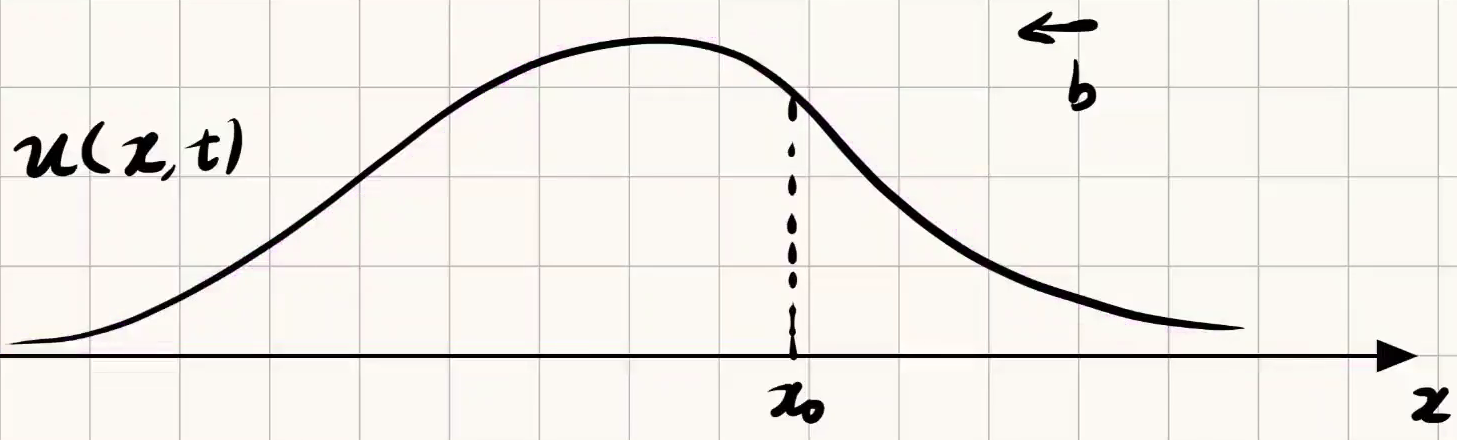
\includegraphics[width=0.5\linewidth]{figure/1.7.1-1}
		\caption{$u(x , t)$ 在某一时刻$t$ 的图像}
		\label{pic : 1.7.1-1} % 添加图像引用标签
	\end{figure}
	
	如图, 固定一个$x_0 \in \R$, $u$ 在该点处沿$b$ 所在方向 ($x$ 轴负方向)的方向导数为正, 因此根据方程
	\[ u_t + b \cdot Du = 0 \]
	$u$ 关于时间的偏导数$u_t$ 在$x_0$ 处的值应为负数, 即在$t + \Delta t$ 时刻, $x_0$ 处的值应减少, 对应如下图像:
	
	\begin{figure}[thbp!]
		\centering
		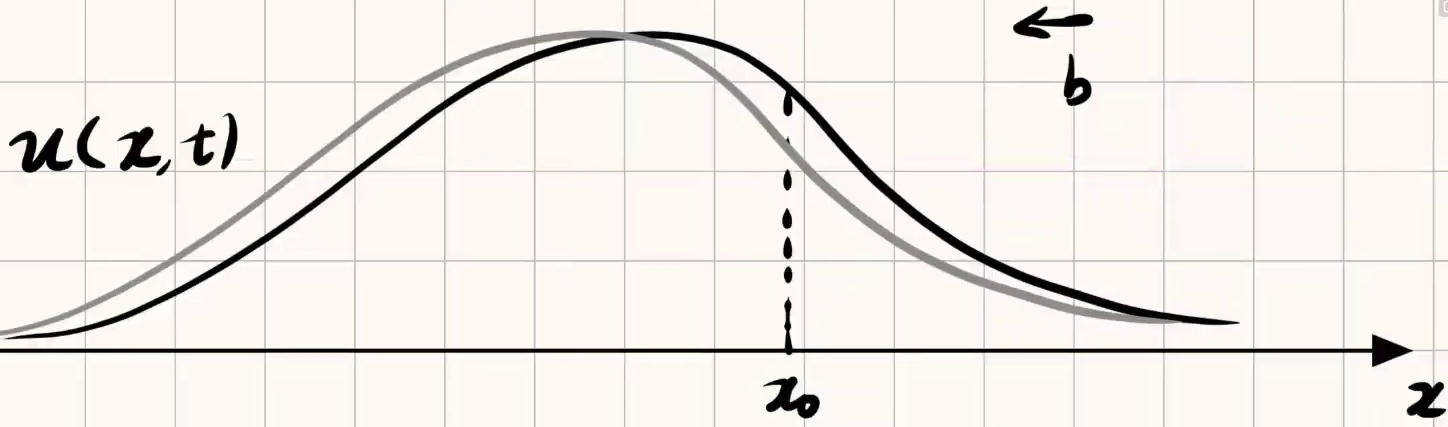
\includegraphics[width=0.5\linewidth]{figure/1.7.1-2}
		\caption{$u(x , t)$ 在时刻$t + \Delta t$ 的图像}
		\label{pic : 1.7.1-2} % 添加图像引用标签
	\end{figure}
	
	其中最高点的函数值保持不变, 此时函数图像随着时间变化就像是被\textbf{“平移”}了, 此即为方程\textbf{“Transport”}名字的几何含义.
	
\newpage

\subsection{特征线法}
\paragraph{猜想}
	在$\S 1.7.1$ 中我们讨论了\textbf{Transport Equation}在几何上随时间的\textbf{“平移性”}. 在这节我们换个更高的角度, 假设方程随时间平移的速度恒定, 则在整个时空$x-t$ 轴上, 每个点的轨迹都应该是一条直线. 即$u$ 在$x-t$ 轴中, 沿着某一固定方向的函数值应当不变, 下面我们就来猜测这样一个方向. \\
	根据方程
	\[ u_t + b \cdot Du = 0 \]
	若想保持$u$ 恒定, 则$u$ 分别沿着$x$ 与$t$ 的行进速率之比应为$\left| b \right| : 1$, 即沿着$(b , 1) \in \R^n \times (0 , \infty)$ 方向移动应当保持恒定. 
	
	\vspace*{1em}
	
	此时在时空$\R^n \times \R = \R^{n + 1}$ 空间中, 就存在着一族平行线, 使得在每一条平行线上$u$ 的函数值均不变. 而此时若得到了某一个与这些线相交的超平面上$u$ 的值, 则可通过平移得到全空间$\R^n \times (0 , \infty)$ 上$u$ 的取值. 下面来证明这一猜想.
	
	\vspace*{6em}
	
	Let
	\begin{align}
		z : \R^n \times (0 , \infty) \times \R &\longrightarrow \R \\
		(x , t , s) &\longmapsto u(x + sb , t + s) = u \Big|_{(x , t) + s(b , 1)}
	\end{align}
	when $(x , t) \in \R^n \times (0 , \infty)$ is fixed we also write $z(x , t , s) = z(s)$. Then
	\begin{align}
		\frac{\partial z}{\partial s} 
		&= \frac{\partial u}{\partial x}(x + sb , t + s) \cdot b + \frac{\partial u}{\partial t}(x + sb , t + s) \\
		&= \left( b \cdot Du + u_{t} \right) \Big|_{(x + sb , t + s)} \\
		&= 0
	\end{align}
	从而$u$ 在每一条沿着$(b , 1) \in \R^n \times (0 , \infty)$ 方向的直线上为常值, 这就证明了我们的猜想. i.e.
	\begin{center}
		$u$ is constant on the line through each $(x , t)$ with direction $(b , 1) \in \R^{n + 1}$.
	\end{center}
	
	\vspace*{4em}
	
	在发现这样一个规律之后, 我们便可以来解决一些初值问题了.
	
\newpage
\paragraph{初值问题}
	\begin{align}
		\begin{cases}
			u_t + b \cdot Du = 0 \hspace*{2em} \text{in} \,\, \R^n \times (0 , \infty) \\
			u(x , 0) = g(x) \hspace*{2em} \text{in} \,\, \R^n \times \{ 0 \}
		\end{cases}
	\end{align}
	where $b \in \R^n$, $g : \R^n \longrightarrow \R$ are known. 
	
	\vspace*{2em}
	
	\begin{rmk}
		上述初值问题事实上给出了$u$ 在$t = 0$ 时的取值, 即给出了时空空间$\R^{n + 1}$ 中超平面$\{ t = 0 \}$ 上的取值. 根据前文中的猜想, $u$ 在全空间$\R^{n + 1}$ 中的取值均可通过沿着$(b , 1)$ 方向的直线平移至该超平面上得到.
	\end{rmk}
	
	\begin{figure}[thbp!]
		\centering
		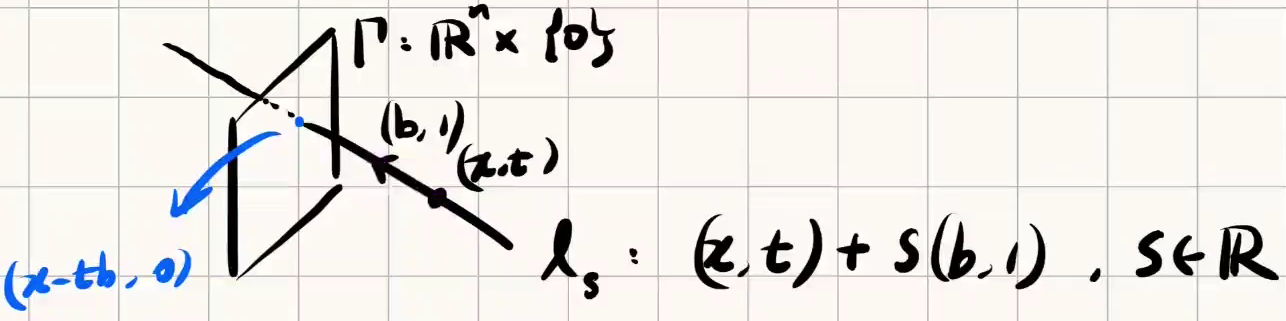
\includegraphics[width=0.7\linewidth]{figure/1.7.2-1}
		\caption{$(x , t)$ 点沿方向$(b , 1)$ 平移至超平面$\{ t = 0 \}$}
		\label{pic : 1.7.2-1} % 添加图像引用标签
	\end{figure}
	
	$\forall (x , t) \in \R^n \times (0 , \infty)$, 设$(x , t) + s(b , 1) = (x + sb , t + s)$, 令$t + s = 0$, 得到:
	\[ s = -t , \,\, x + sb = x - tb \]
	于是$u(x , t) = u(x - tb , 0) = g(x - tb) , \,\, \forall (x , t) \in \R^n \times (0 , \infty)$.
	
\newpage
\paragraph{非齐次初值问题 (Non-homogeneous)}
	上面我们解决了\textbf{齐次初值问题}的求解, 下面我们仍用类似的方法, 求解一般的\textbf{非齐次初值问题}.
	\begin{align}
		\begin{cases}
			u_t + b \cdot Du = f \hspace*{2em} \text{in} \,\, \R^n \times (0 , \infty) \\
			u(x , 0) = g(x) \hspace*{2em} \text{in} \,\, \R^n \times \{ 0 \}
		\end{cases}
	\end{align}
	where $b \in \R^n$, $g : \R^n \longrightarrow \R$ and $f : \R^n \times (0 , \infty) \longrightarrow \R$ are known. 
	
	\vspace*{6em}
	
	\begin{solution}
		此时对于$z(x , t , s) = u(x + sb , t + s) = u \Big|_{(x , t) + s(b , 1)}$, 
		\begin{align}
			\frac{\partial z}{\partial s} 
			&= \frac{\partial u}{\partial x}(x + sb , t + s) \cdot b + \frac{\partial u}{\partial t}(x + ts , t + s) \\
			&= \left( b \cdot Du + u_t \right)\Big|_{(x + sb , t + s)} \\
			&= f(x + sb , t + s)
		\end{align}
		Fix $(x , t) \in \R^n \times (0 , \infty)$. Denote $z(s) = z(x , t , s)$, then
		\begin{align}
			\begin{cases}
				z(0) = u(x , t) \\
				z(-t) = u(x - tb , 0) = g(x - tb)
			\end{cases}
		\end{align}
		Thus
		\[
			z(0) - z(-t) 
			= \int_{-t}^{0} \frac{\partial z}{\partial s}(s) \, ds 
			= \int_{-t}^{0} f(x + sb , t + s) \, ds
		\]
		i.e. for $\forall (x , t) \in \R^n \times (0 , \infty)$
		\begin{align}
			u(x , t) = g(x - tb) + \int_{-t}^{0} f(x + ts , t + s) \, ds 
		\end{align}
	\end{solution}



	%  ############################
	\ifx\allfiles\undefined
\end{document}
\fi